%%%%%%%%%%%%%%%%%%%%%%%%%%%%%%%%%%%%%%%%%

\chapter{Introduction and background}

%%%%%%%%%%%%%%%%%%%%%%%%%%%%%%%%%%%%%%%%%

An electric dipole moment (EDM), $\vv{d}$, is an intrinsic property that describes the effect of an external electric field on the particle. For a neutral particle, it may be naively considered as two point charges $+q$ and $-q$ separated by a distance $\vv{r}$, such that $\vv{d}=q\cdot \vv{r}$. For a general continuous charge distribution $\rho(\vv{r})$ this is written to be
%
\begin{gather}
    \vv{d}=\int d^3r\,\,\vv{r}\rho(\vv{r})
\end{gather}
%
If there is an asymmetry in the charge distribution within the particle, then there is a nonzero EDM. The existence of an EDM violates parity symmetry $P$ and time reversal symmetry $T$ (Sec.~\ref{sec:CP_violation}). Under the $CPT$ theorem, this implies $CP$ violation.

A nonzero EDM has yet to be measured~\cite{CHU19}. The existing bound on the neutron EDM (\acrshort*{nedm}) is $\gls*{d_n}\leq \num{1.8e-26}\,e\,\text{cm (90\% \acrshort{cl})}$~\cite{pdg2022}. A nEDM measurement is one of the most sensitive probes of $CP$ violation, and may give clues to the puzzle of the matter–antimatter asymmetry in the universe (Sec.~\ref{sec:CP_violation_SM}\textendash\ref{sec:history_nedm}).

%%%%%%%%%%%%%%%%%%%%%%%%%%%%%%%%%%%%%%%%%

\section{CP violation}\label{sec:CP_violation}

%%%%%%%%%%%%%%%%%%%%%%%%%%%%%%%%%%%%%%%%%

\begin{table}
\centering
\caption[Transformations of relevant physical observables under $C$, $P$, and $T$ operations]{\label{tb:cpt_transform}Transformations under $C$, $P$, and $T$ operations}
\begin{tabular}{lllll}
\toprule
& & $C$ & $P$ & $T$ \\ 
\midrule
$\vv{r}$ & Position & $+$ & $-$ & $+$ \\
$t$ & Time & $+$ & $+$ & $-$ \\
$\vv{p}$ & Momentum & $+$ & $-$ & $-$ \\
$\vv{S}$ & Spin & $+$ & $+$ & $-$ \\
$\vv{\mu}$ & Magnetic dipole moment  & $-$ & $+$ & $-$ \\
$\vv{d}$ & Electric dipole moment  & $-$ & $+$ & $-$ \\
$\vv{B}$ & Magnetic field  & $-$ & $+$ & $-$ \\
$\vv{E}$ & Electric field & $-$ & $-$ & $+$ \\
\bottomrule
\end{tabular}
\end{table}


A physical law, process, or quantity is symmetric under a certain operation if it remains unchanged by the operation. Three discrete symmetries play a critical role in fundamental physics: charge conjugation $C$, parity inversion $P$, and time reversal $T$.

Tab.~\ref{tb:cpt_transform} contains a summary of transformations under $C$, $P$, and $T$. Here, ``$+$'' denotes that the quantity is even (invariant) under the transformation, and ``$-$'' denotes that the quantity is odd under the transformation.

Charge conjugation transforms all charge quantum numbers of a particle. This includes electrical charge, color charge, lepton or baryon number, etc. $C$ converts a particle into its anti-particle. Classical electrodynamics is invariant under $C$. The potentials and fields all change signs, leaving the forces unaffected.

Parity, or spatial inversion, changes the sign of all spatial Cartesian coordinates. It is equivalent to reflection in a plane (mirror symmetry). A quantity such as classical linear momentum transforms as $\vv{p}\xrightarrow{P} -\vv{p}$. An example of a quantity invariant under $P$ is spin $1/2$. To provide intuition as to why this is true, consider the classical angular momentum definition $\vv{r} \times \vv{p}$. The cross product of two polar vectors is an axial vector (or pseudovector) that does not change under $P$ (as seen by $(-\vv{r}) \times (-\vv{p}) = \vv{r} \times \vv{p}$).

Parity violation in the weak interaction was proposed by Lee and Yang in 1956 \cite{lee_yang_1956} to explain the $\theta$\textendash$\tau$ problem and subsequently observed by Wu et al.~\cite{wu_1956}. Wu and his collaborators polarized nuclear spins of $\ce{^{60}Co}$ with a magnetic field and measured the angular distribution of the electrons from $\beta$ decay. They found that electrons were preferentially emitted in the direction opposite to the polarization of the spin, violating parity. Written mathematically, the quantity $\vv{S}\cdot\vv{p}_e$, which describes the angular distribution of emission, transforms as $\vv{S}\cdot\vv{p}_e \xrightarrow{P} \vv{S}\cdot(-\vv{p}_e) \neq \vv{S}\cdot\vv{p}_e$. We define a pseudoscalar as a quantity that behaves as a scalar but changes under $P$, such as $\vv{S}\cdot\vv{p}_e$.

Time reversal performs the transformation $t \xrightarrow{T} -t$. An example of a process invariant under $T$ is a classical elastic collision of billiard balls, where watching a video of the process played backwards would be identical to the video in normal time. A quantity such as spin, however, changes sign under $T$ similar to how the angular momentum vector of a gyroscope changes when the direction of rotation changes.

In quantum mechanics the the time reversal operator performs both time reversal and complex conjugation. To demonstrate, we consider the \schrodinger equation for a spin 0 system in an external scalar potential
%
\begin{gather}
    i\hbar\frac{\partial \psi}{\partial t} = \left(-\frac{\hbar^2}{2m}\nabla^2 + V \right) \psi
\end{gather}
%
Let $\psi(\vv{x}, t)=u_n(\vv{x})\exp(-iE_nt/\hbar)$ be a solution. If we desire the system to be symmetric under $T$, $\psi(\vv{x}, -t)$ cannot be a solution due to the time derivative on the left hand side of the equation. However, $\psi^*(\vv{x}, -t)=u_n^*(\vv{x})\exp(-iE_nt/\hbar)$ is viable.

Let us examine the behavior of a particle with both electric $(\vv{d})$ and magnetic $(\vv{\mu})$ dipole moments in the presence of external magnetic $(\vv{B})$ and electric $(\vv{E})$ fields under transformations $P$ and $T$. In the nonrelativistic limit, the interaction Hamiltonian is 
%
\begin{gather}
    H_\text{EDM} = -\vv{d}\cdot\vv{E}-\vv{\mu}\cdot\vv{B} \label{eq:edm_hamiltonian}
\end{gather}
%
where by the Wigner-Ekart theorem~\cite{sakurai_quantum}, the EDM of a spin $1/2$ particle must be colinear to the spin $\vv{S}$. This allows us to write $\vv{\mu}=\mu\vv{S}$ and $\vv{d}=\delta\vv{S}$. Therefore, dipole moment operators transform under $P$ and $T$ the same as spin, an axial vector.

Under $P$, the polar vector $\vv{E}$ changes sign when the locations of all charges are inverted. However, there is no explicit time dependence in $\vv{E}$, so under $T$ there is no change. In contrast, under $P$ the magnetic field does not change. Intuitively, we observe that the Biot-Savart Law defined by $d\vv{B}\propto I\,d\vec{l} \times \hat{r} /r^2$ contains a cross product, an axial vector. However, $\vv{B}$ is $T$-odd because the directions of all currents are reversed while the spatial configuration stays the same. 

Applying $P$ to Eq.~(\ref{eq:edm_hamiltonian}) we immediately see
%
\begin{gather}
    H_\text{EDM}\xrightarrow{P} -\vv{d}\cdot(-\vv{E}) - \vv{\mu}\cdot\vv{B} \neq H_\text{EDM}
\end{gather}
%
and under $T$ we have
%
\begin{gather}
    H_\text{EDM}\xrightarrow{T} -(-\vv{d})\cdot\vv{E} - (-\vv{\mu})\cdot(-\vv{B}) \neq H_\text{EDM}
\end{gather}
%
The EDM interaction with external fields violates $T$ and $P$ symmetries. 

The $CPT$ theorem states that any locally Lorentz-covariant field theory of a point like particle is $CPT$ invariant \cite{LUDERS19571, schmidt-wellenburg_quest_2017, cp_violation_wo_strangeness}. In other words, the $CPT$ theorem arises from Lorentz invariance and locality; the Lorentz-invariant Hamiltonian must be invariant under the operations $C$, $P$, and $T$ combined. $CPT$ symmetry implies that when $T$ is violated, $CP$ must also be violated. Therefore the $T$-odd EDM is directly related to $CP$ violation. In 1964, $CP$ violation was observed in $K^0$ decay~\cite{christenson_1964}, stimulating interests in EDMs and other $T$-odd processes.

%%%%%%%%%%%%%%%%%%%%%%%%%%%%%%%%%%%%%%%%%

\subsection{Induced nEDM}

%%%%%%%%%%%%%%%%%%%%%%%%%%%%%%%%%%%%%%%%%

As a composite system made of quarks and gluons, due to an internal charge distribution, a neutron subjected to an external electric field creates an induced nEDM given by $d_\text{induced}=4\pi \epsilon_0 \alpha_\text{n} E$. Unlike the permanent nEDM $\gls{d_n}$, the induced nEDM is not constrained by the Wigner-Eckhart theorem to be colinear to the spin vector, and does not violate $P$ and $T$.

The neutron polarizability $\alpha_\text{n}$ is $(11.8\pm 1.1)\,10^{-4}\text{ fm}^3$~\cite{pdg2022}, giving a value $d_\text{induced}\sim 10^{-32}e\,\text{cm}$ for $E=\qty{10}{kV\per cm}$. This is well below current experimental limits (Sec.~\ref{fig:nEDM-history}). In addition, the spin dependent interactions described in Chap.~\ref{chap:spinManipulation} are independent of polarizability, such that typical nEDM measurement techniques (Sec.~\ref{sec:ramsey-method}) are insensitive to the induced nEDM. 

Reference~\cite{baym_elementary_2016} examines the induced nEDM in further detail, including a derivation where the ratio $\gls*{d_n}/d_\text{induced}$ is related to a general $CP$ violating term.

%%%%%%%%%%%%%%%%%%%%%%%%%%%%%%%%%%%%%%%%%

\section{CP violation and the nEDM in the Standard Model}\label{sec:CP_violation_SM}

%%%%%%%%%%%%%%%%%%%%%%%%%%%%%%%%%%%%%%%%%

\begin{figure}[htp]
    \centering
    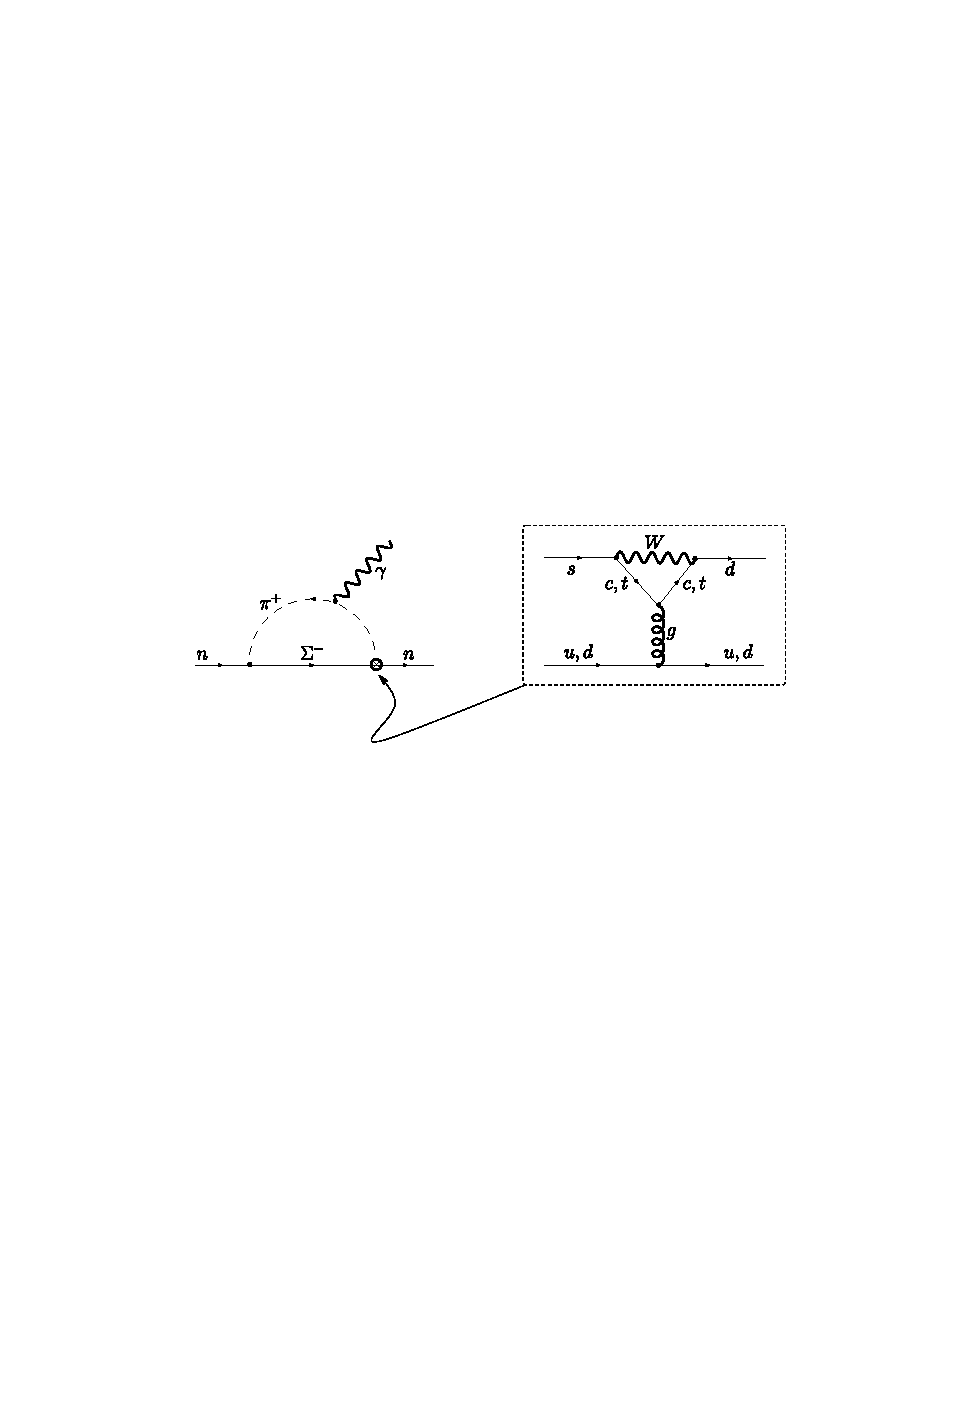
\includegraphics[width=0.6\textwidth]{figures/Pospelov_strong_penguin.pdf}
    \caption[The strong penguin diagram, the largest $CP$ violating phase contribution to the nEDM in the SM]
    {The strong penguin diagram (crossed vertex), the largest $CP$ violating phase contribution to the nEDM in the SM. Image from \cite{POS05}}
    \label{fig:strong_penguin}
\end{figure}

There are two known sources of $CP$ violation in the Standard Model (\acrshort*{sm}). The first is found in the electroweak sector, via the Cabbibo-Kobayashi-Maskawa (CKM) matrix, which describes a rotation between weak eigenstates and flavor eigenstates, as observed in charge-current weak decay processes~\cite{ckm1973, ChauKeung1984, pdg2022}.
%
\begin{align}
    V_\text{CKM} &= \left( \begin{matrix}
    V_\text{ud} & V_\text{us} & V_\text{ub} \\
    V_\text{cd} & V_\text{cs} & V_\text{cb} \\
    V_\text{td} & V_\text{ts} & V_\text{tb} \\
    \end{matrix} \right) \label{eq:CKM} \\
    &= \left( \begin{matrix}
    c_{12}c_{13} & s_{12}c_{13} & s_{13}e^{-i\delta} \\
    -s_{12}c_{23}-c_{12}s_{23}s_{13}e^{i\delta} & c_{12}c_{23}-s_{12}s_{23}s_{13}e^{i\delta} & s_{23}c_{13} \\
    s_{12}s_{23}-c_{12}c_{23}s_{13}e^{i\delta} & -c_{12}s_{23}s_{13}e^{i\delta} & c_{23}c_{13} \\
    \end{matrix} \right)
\end{align}
%
where $c_{ij}=\cos\theta_{ij}$, $s_{ij}=\sin\theta_{ij}$, and $\delta\approx1.2\text{ rad}$ is the $CP$ violating phase.

As far as we know, $V_\text{CKM}$ is unitary $(V_\text{CKM}V_\text{CKM}^\dag=I)$. For a $3 \times 3$ unitary matrix, the nine unknown complex elements of $V_{ij}$ may be reduced to three real numbers (rotation angle $\theta_{ij}$) and one complex phase factor ($e^{i\delta}$), where the complex phase accounts for $CP$ violation.

We now examine contributions to the nEDM in the SM, beginning with quark EDMs. The neutron is a composite object consisting of three valence quarks ($udd$) and a sea of gluons and mesons. At tree level, there is no diagram generating a $CP$-violating EDM interaction of one quark of the neutron with an electric field. At one loop, each CKM matrix element comes with a complex conjugate, thus negating any $CP$ violating phase. At the two loop level, the sum over all quark flavors in intermediate states still leads to a vanishing EDM \cite{schmidt-wellenburg_quest_2017, czarnecki_valence_model_1997}.

In fact, the quark EDM appears only starting at the three loop level, with the largest effect from the exchange of two W bosons and one gluon. Taking a simplified valence approach to estimating the nEDM gives \cite{czarnecki_valence_model_1997}
%
\begin{gather}
    \gls*{d_n}^\text{valence} = \frac{4}{3}d_d - \frac{1}{3}d_u \lesssim 10^{-34}\,e\text{ cm}
\end{gather}

The largest $CP$ violating phase contribution to the nEDM arises from the so-called strong penguin diagram (Fig.~\ref{fig:strong_penguin}) \cite{POS05}. The contribution to a nEDM is enhanced by a long distance $\pi^-$ loop, and it is estimated to be
%
\begin{gather}
    \gls*{d_n}^\text{penguin} \sim 10^{-32}\,e\text{ cm}
\end{gather}
%
This is 6 orders of magnitude lower than current experimental limits on the nEDM ($\sim 10^{-26}\,e\text{ cm}$ \cite{ABE20}). Improvements to nEDM measurements are effective probes of new physics beyond the Standard Model (\acrshort*{bsm}).

%%%%%%%%%%%%%%%%%%%%%%%%%%%%%%%%%%%%%%%%%

\subsection{Strong CP problem}

%%%%%%%%%%%%%%%%%%%%%%%%%%%%%%%%%%%%%%%%%

The second source of $CP$ violation in the SM comes from the quantum chromodynamics (QCD) Lagrangian term for the strong interaction. The $CP$ violating dimension-4 operator is
%
\begin{gather}
    \mathcal{L}_\text{QCD}^\text{CP\textendash odd}=\frac{g^2_s}{32\pi^2}\overline{\theta}G^a_{\mu\nu}\tilde{G}^{\mu\nu, a}
\end{gather}
%
where $g_s$ is the strong interaction coupling, $\overline{\theta}$ is the $CP$ violating phase, and $G^a_{\mu\nu}$ is the QCD gluon field tensor. It provides an nEDM contribution on the order of \cite{cp_violation_wo_strangeness}
%
\begin{gather}
    \gls*{d_n}^\text{QCD}\sim \overline{\theta}\times 10^{-16}\,e\text{ cm}
\end{gather}
%
Current experimental limits imply that $\overline{\theta}\lesssim 10^{-10}$, an arbitrarily tiny number given that the phase $\overline{\theta}$ has a permissible range $[0, 2\pi]$. There is no inherent reasoning as to why $\overline{\theta}$ is so small, resulting in the ``strong $CP$ problem.''

One proposed solution to the strong $CP$ problem is to introduce a Peccei-Quinn symmetry, which resulted in a Goldstone boson called the axion \cite{peccei_quinn_axion}, a dark matter candidate. See Refs.~\cite{BAER20151, kim_gianpaolo_2010} for reviews on the topic.

%%%%%%%%%%%%%%%%%%%%%%%%%%%%%%%%%%%%%%%%%

\section{Baryon asymmetry of the universe}

%%%%%%%%%%%%%%%%%%%%%%%%%%%%%%%%%%%%%%%%%

$CP$ symmetry implies that for any particle there should be an antiparticle of equal mass, decay width, and opposite charge. Particles and antiparticles should have equal distributions at thermal equilibrium. By these symmetry arguments, one would reasonably expect that the universe should contain equal amounts of particles and antiparticles, or that particles and antiparticles mostly annihilated during the early universe and are now very sparse.

In reality, this is not the case, and matter is heavily dominant. Estimates based on the Standard Model of the expected baryon matter/anti-matter asymmetry in the universe (\acrshort*{bau}) is 8 orders of magnitude smaller than the baryon-to-photon ratio observed using the cosmic microwave background (CMB) \cite{Mor13, Dubbers2011}.

Sakharov \cite{Sakharov_1991} first suggested 3  necessary conditions for baryogenesis, the production of BAU from an initally symmetric state in the early universe. The Sakharov criteria are:
%
\begin{enumerate}
    \item Baryon number violation: For some initial baryon number $B=0$ there must be some interaction that violates baryon number to proceed to a universe with a net $B>0$.
    \item $C$ and $CP$ violation: If $C$ and $CP$ are exact symmetries, then the probability of converting matter to antimatter is the same as the reverse process, resulting in $B=0$.
    \item Breaking of thermal equilibrium:  At thermal equilibrium, there is no preferred direction for time and $CPT$ invariance prevents baryon excess, negating the effect of any $CP$ violating processes.
\end{enumerate}

In the SM, there is an insufficient departure from thermal equilibrium and too little $CP$ violation for baryogenesis to be permitted. Reference~\cite{Dubbers2011} describes this in further detail.

%%%%%%%%%%%%%%%%%%%%%%%%%%%%%%%%%%%%%%%%%

\section{Beyond standard model physics}

%%%%%%%%%%%%%%%%%%%%%%%%%%%%%%%%%%%%%%%%%

\begin{figure}
    \centering
    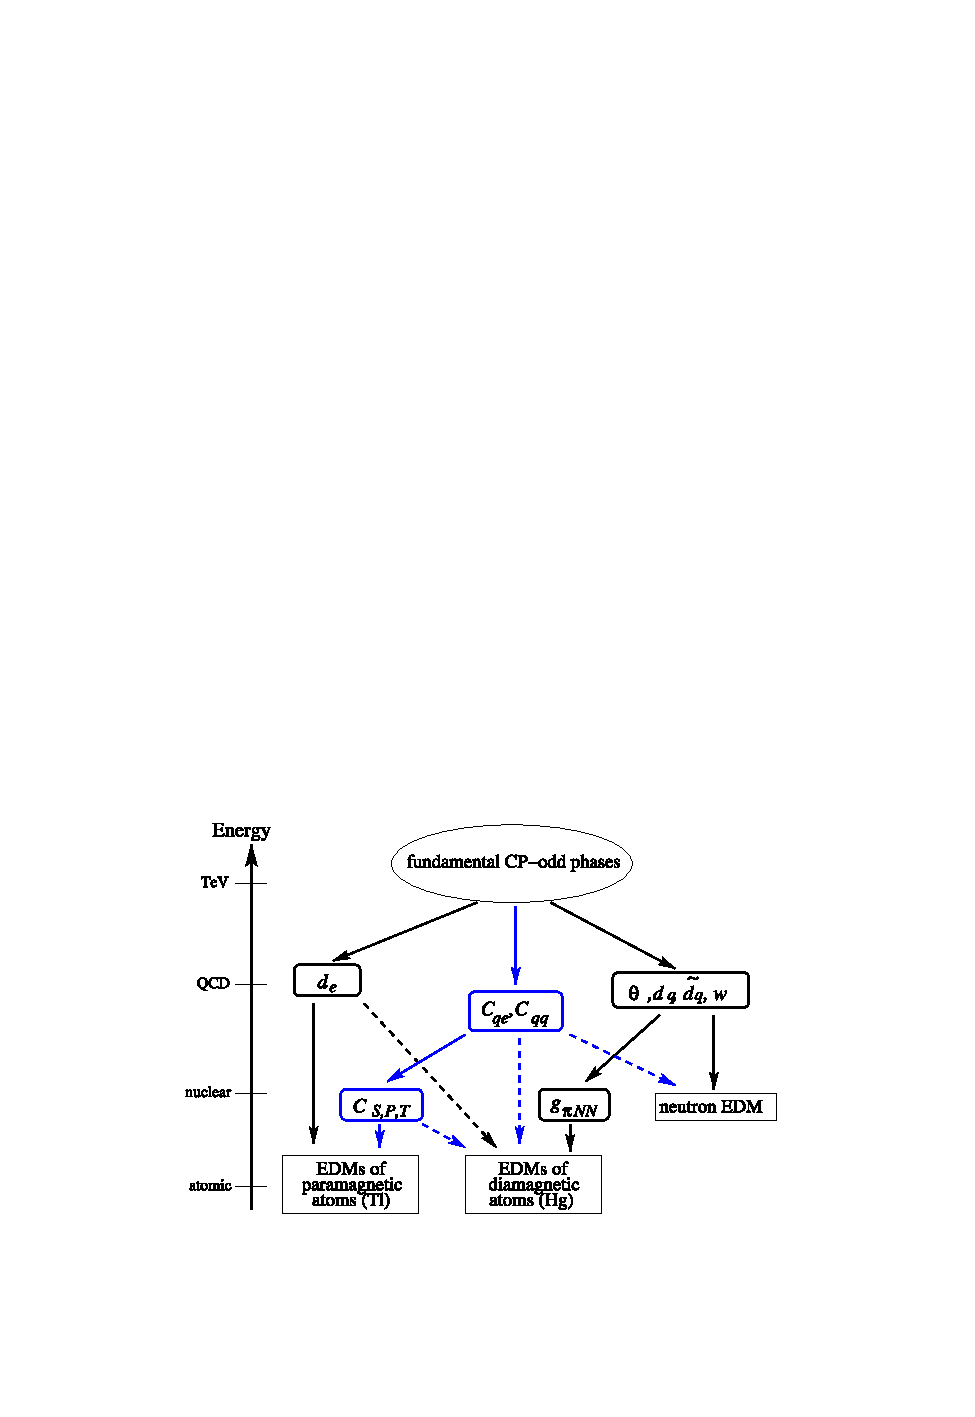
\includegraphics[height=3in]{figures/Pospelov_BSM_CPV.pdf}
    \caption[A hierarchy of scales between BSM $CP$ violating sources and 3 general types of EDM observables.]
    {A hierarchy of scales between BSM $CP$ violating sources and 3 general types of EDM observables. Dashed lines depict weaker dependencies. Image from Ref. \cite{POS05}.}
    \label{fig:bsm_cp_violation}
\end{figure}

Physics beyond the SM (\acrshort{bsm}) is required for additional sources of $CP$ violation. For nEDM and EDM experiments, $CP$ violating contributions from the SM are effectively background, making EDMs very sensitive tests of BSM physics. Most SM extensions treat the SM as the low energy limit of a higher framework. $CP$\textendash odd parameters propagate from a $\sim$\unit{\tera\eV} scale down to a low energy observable (Fig.~\ref{fig:bsm_cp_violation}). Unfortunately, extracting a $CP$ violating phase from such an observable becomes difficult, requiring cross references of multiple EDM measurements. For reviews on new sources of $CP$ violation see Refs.~\cite{Cir10, POS05, ENG13, CHU19}.

%%%%%%%%%%%%%%%%%%%%%%%%%%%%%%%%%%%%%%%%%

\section{A brief history of nEDM experiments}\label{sec:history_nedm}

%%%%%%%%%%%%%%%%%%%%%%%%%%%%%%%%%%%%%%%%%

The first nEDM experiment was begun by Ramsey and Purcell in 1950, with the first result published in 1957 \cite{ramsey_nedm_1950, ramsey_nedm_1957}. The upper bound on $\gls*{d_n}$ has decreased steadily ever since (Fig.~\ref{fig:nEDM-history}). Early nEDM measurements \cite{miller_nedm_1967, baird_nedm_1969, cohen_nedm_1969} used thermal neutrons (\num{10000} to \qty{50000}{\micro \eV}) passing a meter-scale apparatus. Subsequent iterations \cite{dress_nedm_1977} shifted to the use of a cold neutron beam (\num{50} to \qty{10000}{\micro \eV}). The sensitivity of beam nEDM measurements was primarily limited by a $\vv{v}\times\vv{E}$ systematic effect (Sec.~\ref{sec:v_cross_E}).

By 1980, nEDM experiments \cite{altarev_nedm_1980, altarev_nedm_1981} began using ultracold neutrons (\ucn), which have kinetic energies $\leq \qty{300}{\nano\eV}$. This enabled measurements with neutrons stored in material bottles \cite{smith_nedm_1990} (see Chap.~\ref{chap:UCN} for properties of \ucn). Lower \ucn velocities and a population-averaged velocity of almost zero mitigated $\vv{v}\times\vv{E}$ systematics (Sec.~\ref{sec:v_cross_E}). 

nEDM experiments continued to improve with increased densities of stored \ucn, advances in magnetic shielding, and more sensitive magnetometry. One significant innovation was the introduction of a cohabitating comagnetomer, a population of $\ce{^{199}Hg}$ atoms that occupied the same space as \ucn, which assists with monitoring magnetic field drifts within the storage volume (Sec.~\ref{sec:199hg_comag}). 

Most nEDM experiments (including beam measurements) use the same measurement principle, the Ramsey method of oscillatory fields \cite{ramsey_molecular_1950}. This technique is described in Chap.~\ref{chap:spinManipulation}. 

The current upper limit on the nEDM has been set by an experiment performed at the Paul Scherrer Institute ($\gls*{d_n}\leq \num{1.8e-26}\,e\,\text{cm [90\% \acrshort{cl}]}$)~\cite{ABE20} and there are several efforts worldwide aimed at searching for the nEDM with improved sensitivity~\cite{Alarcon2022}. The nEDM experiment at \acrlong*{lanl} (\acrshort*{lanl}) will use the Ramsey method to search for the nEDM with an uncertainty goal of $\delta \gls*{d_n} = \num{2e-27}\,e\text{ cm}$.

\begin{figure}
    \centering
    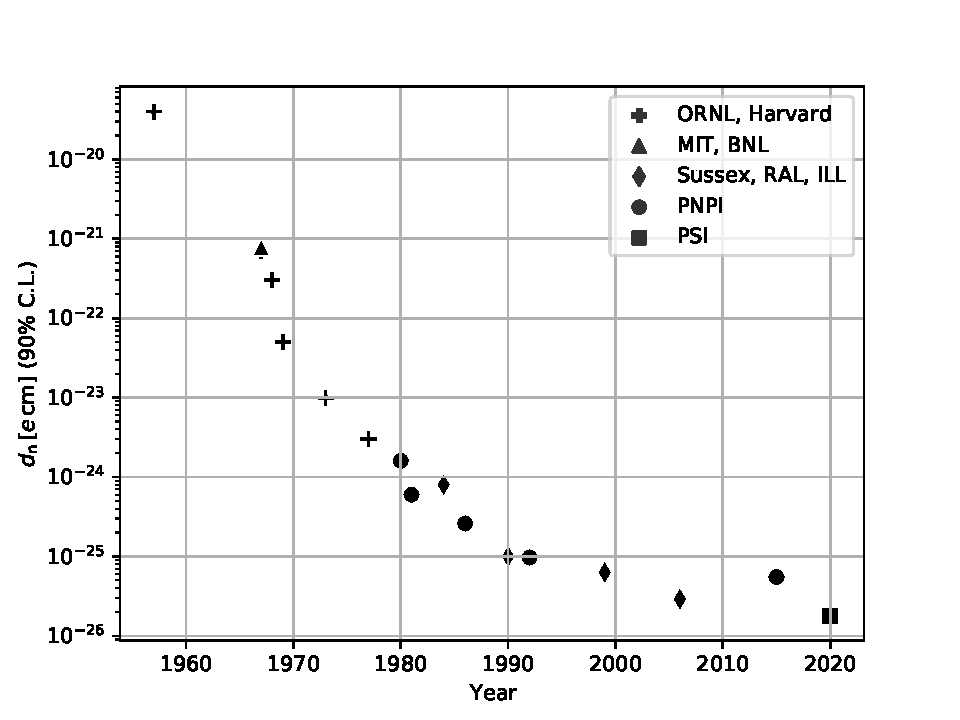
\includegraphics[height=3.5in]{figures/nEDM-history.pdf}
    \caption[History of published nEDM measurements and the institutions involved.]{History of published nEDM measurements and the institutions involved. See Refs.~\cite{ramsey_nedm_1950, ramsey_nedm_1957, miller_nedm_1967, shull_nedm_1967, dress_nedm_1968, cohen_nedm_1969, dress_nedm_1973, dress_nedm_1977, altarev_nedm_1980, altarev_nedm_1981, pendlebury_nedm_1984,
    altarev_nedm_1986, smith_nedm_1990, altarev_nedm_1992, altarev_nedm_1996, harris_nedm_1999, BAK06, ABE20, pnpi_nedm_2015}. The vertical dotted line refers to the measurement of $CP$ violation in $K^0$ decay~\cite{christenson_1964}.}
    \label{fig:nEDM-history}
\end{figure}